
\documentclass{article} % For LaTeX2e
\usepackage{iclr2020_conference,times}

% Optional math commands from https://github.com/goodfeli/dlbook_notation.
%%%%% NEW MATH DEFINITIONS %%%%%

\usepackage{amsmath,amsfonts,bm}

% Mark sections of captions for referring to divisions of figures
\newcommand{\figleft}{{\em (Left)}}
\newcommand{\figcenter}{{\em (Center)}}
\newcommand{\figright}{{\em (Right)}}
\newcommand{\figtop}{{\em (Top)}}
\newcommand{\figbottom}{{\em (Bottom)}}
\newcommand{\captiona}{{\em (a)}}
\newcommand{\captionb}{{\em (b)}}
\newcommand{\captionc}{{\em (c)}}
\newcommand{\captiond}{{\em (d)}}

% Highlight a newly defined term
\newcommand{\newterm}[1]{{\bf #1}}


% Figure reference, lower-case.
\def\figref#1{figure~\ref{#1}}
% Figure reference, capital. For start of sentence
\def\Figref#1{Figure~\ref{#1}}
\def\twofigref#1#2{figures \ref{#1} and \ref{#2}}
\def\quadfigref#1#2#3#4{figures \ref{#1}, \ref{#2}, \ref{#3} and \ref{#4}}
% Section reference, lower-case.
\def\secref#1{section~\ref{#1}}
% Section reference, capital.
\def\Secref#1{Section~\ref{#1}}
% Reference to two sections.
\def\twosecrefs#1#2{sections \ref{#1} and \ref{#2}}
% Reference to three sections.
\def\secrefs#1#2#3{sections \ref{#1}, \ref{#2} and \ref{#3}}
% Reference to an equation, lower-case.
\def\eqref#1{equation~\ref{#1}}
% Reference to an equation, upper case
\def\Eqref#1{Equation~\ref{#1}}
% A raw reference to an equation---avoid using if possible
\def\plaineqref#1{\ref{#1}}
% Reference to a chapter, lower-case.
\def\chapref#1{chapter~\ref{#1}}
% Reference to an equation, upper case.
\def\Chapref#1{Chapter~\ref{#1}}
% Reference to a range of chapters
\def\rangechapref#1#2{chapters\ref{#1}--\ref{#2}}
% Reference to an algorithm, lower-case.
\def\algref#1{algorithm~\ref{#1}}
% Reference to an algorithm, upper case.
\def\Algref#1{Algorithm~\ref{#1}}
\def\twoalgref#1#2{algorithms \ref{#1} and \ref{#2}}
\def\Twoalgref#1#2{Algorithms \ref{#1} and \ref{#2}}
% Reference to a part, lower case
\def\partref#1{part~\ref{#1}}
% Reference to a part, upper case
\def\Partref#1{Part~\ref{#1}}
\def\twopartref#1#2{parts \ref{#1} and \ref{#2}}

\def\ceil#1{\lceil #1 \rceil}
\def\floor#1{\lfloor #1 \rfloor}
\def\1{\bm{1}}
\newcommand{\train}{\mathcal{D}}
\newcommand{\valid}{\mathcal{D_{\mathrm{valid}}}}
\newcommand{\test}{\mathcal{D_{\mathrm{test}}}}

\def\eps{{\epsilon}}


% Random variables
\def\reta{{\textnormal{$\eta$}}}
\def\ra{{\textnormal{a}}}
\def\rb{{\textnormal{b}}}
\def\rc{{\textnormal{c}}}
\def\rd{{\textnormal{d}}}
\def\re{{\textnormal{e}}}
\def\rf{{\textnormal{f}}}
\def\rg{{\textnormal{g}}}
\def\rh{{\textnormal{h}}}
\def\ri{{\textnormal{i}}}
\def\rj{{\textnormal{j}}}
\def\rk{{\textnormal{k}}}
\def\rl{{\textnormal{l}}}
% rm is already a command, just don't name any random variables m
\def\rn{{\textnormal{n}}}
\def\ro{{\textnormal{o}}}
\def\rp{{\textnormal{p}}}
\def\rq{{\textnormal{q}}}
\def\rr{{\textnormal{r}}}
\def\rs{{\textnormal{s}}}
\def\rt{{\textnormal{t}}}
\def\ru{{\textnormal{u}}}
\def\rv{{\textnormal{v}}}
\def\rw{{\textnormal{w}}}
\def\rx{{\textnormal{x}}}
\def\ry{{\textnormal{y}}}
\def\rz{{\textnormal{z}}}

% Random vectors
\def\rvepsilon{{\mathbf{\epsilon}}}
\def\rvtheta{{\mathbf{\theta}}}
\def\rva{{\mathbf{a}}}
\def\rvb{{\mathbf{b}}}
\def\rvc{{\mathbf{c}}}
\def\rvd{{\mathbf{d}}}
\def\rve{{\mathbf{e}}}
\def\rvf{{\mathbf{f}}}
\def\rvg{{\mathbf{g}}}
\def\rvh{{\mathbf{h}}}
\def\rvu{{\mathbf{i}}}
\def\rvj{{\mathbf{j}}}
\def\rvk{{\mathbf{k}}}
\def\rvl{{\mathbf{l}}}
\def\rvm{{\mathbf{m}}}
\def\rvn{{\mathbf{n}}}
\def\rvo{{\mathbf{o}}}
\def\rvp{{\mathbf{p}}}
\def\rvq{{\mathbf{q}}}
\def\rvr{{\mathbf{r}}}
\def\rvs{{\mathbf{s}}}
\def\rvt{{\mathbf{t}}}
\def\rvu{{\mathbf{u}}}
\def\rvv{{\mathbf{v}}}
\def\rvw{{\mathbf{w}}}
\def\rvx{{\mathbf{x}}}
\def\rvy{{\mathbf{y}}}
\def\rvz{{\mathbf{z}}}

% Elements of random vectors
\def\erva{{\textnormal{a}}}
\def\ervb{{\textnormal{b}}}
\def\ervc{{\textnormal{c}}}
\def\ervd{{\textnormal{d}}}
\def\erve{{\textnormal{e}}}
\def\ervf{{\textnormal{f}}}
\def\ervg{{\textnormal{g}}}
\def\ervh{{\textnormal{h}}}
\def\ervi{{\textnormal{i}}}
\def\ervj{{\textnormal{j}}}
\def\ervk{{\textnormal{k}}}
\def\ervl{{\textnormal{l}}}
\def\ervm{{\textnormal{m}}}
\def\ervn{{\textnormal{n}}}
\def\ervo{{\textnormal{o}}}
\def\ervp{{\textnormal{p}}}
\def\ervq{{\textnormal{q}}}
\def\ervr{{\textnormal{r}}}
\def\ervs{{\textnormal{s}}}
\def\ervt{{\textnormal{t}}}
\def\ervu{{\textnormal{u}}}
\def\ervv{{\textnormal{v}}}
\def\ervw{{\textnormal{w}}}
\def\ervx{{\textnormal{x}}}
\def\ervy{{\textnormal{y}}}
\def\ervz{{\textnormal{z}}}

% Random matrices
\def\rmA{{\mathbf{A}}}
\def\rmB{{\mathbf{B}}}
\def\rmC{{\mathbf{C}}}
\def\rmD{{\mathbf{D}}}
\def\rmE{{\mathbf{E}}}
\def\rmF{{\mathbf{F}}}
\def\rmG{{\mathbf{G}}}
\def\rmH{{\mathbf{H}}}
\def\rmI{{\mathbf{I}}}
\def\rmJ{{\mathbf{J}}}
\def\rmK{{\mathbf{K}}}
\def\rmL{{\mathbf{L}}}
\def\rmM{{\mathbf{M}}}
\def\rmN{{\mathbf{N}}}
\def\rmO{{\mathbf{O}}}
\def\rmP{{\mathbf{P}}}
\def\rmQ{{\mathbf{Q}}}
\def\rmR{{\mathbf{R}}}
\def\rmS{{\mathbf{S}}}
\def\rmT{{\mathbf{T}}}
\def\rmU{{\mathbf{U}}}
\def\rmV{{\mathbf{V}}}
\def\rmW{{\mathbf{W}}}
\def\rmX{{\mathbf{X}}}
\def\rmY{{\mathbf{Y}}}
\def\rmZ{{\mathbf{Z}}}

% Elements of random matrices
\def\ermA{{\textnormal{A}}}
\def\ermB{{\textnormal{B}}}
\def\ermC{{\textnormal{C}}}
\def\ermD{{\textnormal{D}}}
\def\ermE{{\textnormal{E}}}
\def\ermF{{\textnormal{F}}}
\def\ermG{{\textnormal{G}}}
\def\ermH{{\textnormal{H}}}
\def\ermI{{\textnormal{I}}}
\def\ermJ{{\textnormal{J}}}
\def\ermK{{\textnormal{K}}}
\def\ermL{{\textnormal{L}}}
\def\ermM{{\textnormal{M}}}
\def\ermN{{\textnormal{N}}}
\def\ermO{{\textnormal{O}}}
\def\ermP{{\textnormal{P}}}
\def\ermQ{{\textnormal{Q}}}
\def\ermR{{\textnormal{R}}}
\def\ermS{{\textnormal{S}}}
\def\ermT{{\textnormal{T}}}
\def\ermU{{\textnormal{U}}}
\def\ermV{{\textnormal{V}}}
\def\ermW{{\textnormal{W}}}
\def\ermX{{\textnormal{X}}}
\def\ermY{{\textnormal{Y}}}
\def\ermZ{{\textnormal{Z}}}

% Vectors
\def\vzero{{\bm{0}}}
\def\vone{{\bm{1}}}
\def\vmu{{\bm{\mu}}}
\def\vtheta{{\bm{\theta}}}
\def\va{{\bm{a}}}
\def\vb{{\bm{b}}}
\def\vc{{\bm{c}}}
\def\vd{{\bm{d}}}
\def\ve{{\bm{e}}}
\def\vf{{\bm{f}}}
\def\vg{{\bm{g}}}
\def\vh{{\bm{h}}}
\def\vi{{\bm{i}}}
\def\vj{{\bm{j}}}
\def\vk{{\bm{k}}}
\def\vl{{\bm{l}}}
\def\vm{{\bm{m}}}
\def\vn{{\bm{n}}}
\def\vo{{\bm{o}}}
\def\vp{{\bm{p}}}
\def\vq{{\bm{q}}}
\def\vr{{\bm{r}}}
\def\vs{{\bm{s}}}
\def\vt{{\bm{t}}}
\def\vu{{\bm{u}}}
\def\vv{{\bm{v}}}
\def\vw{{\bm{w}}}
\def\vx{{\bm{x}}}
\def\vy{{\bm{y}}}
\def\vz{{\bm{z}}}

% Elements of vectors
\def\evalpha{{\alpha}}
\def\evbeta{{\beta}}
\def\evepsilon{{\epsilon}}
\def\evlambda{{\lambda}}
\def\evomega{{\omega}}
\def\evmu{{\mu}}
\def\evpsi{{\psi}}
\def\evsigma{{\sigma}}
\def\evtheta{{\theta}}
\def\eva{{a}}
\def\evb{{b}}
\def\evc{{c}}
\def\evd{{d}}
\def\eve{{e}}
\def\evf{{f}}
\def\evg{{g}}
\def\evh{{h}}
\def\evi{{i}}
\def\evj{{j}}
\def\evk{{k}}
\def\evl{{l}}
\def\evm{{m}}
\def\evn{{n}}
\def\evo{{o}}
\def\evp{{p}}
\def\evq{{q}}
\def\evr{{r}}
\def\evs{{s}}
\def\evt{{t}}
\def\evu{{u}}
\def\evv{{v}}
\def\evw{{w}}
\def\evx{{x}}
\def\evy{{y}}
\def\evz{{z}}

% Matrix
\def\mA{{\bm{A}}}
\def\mB{{\bm{B}}}
\def\mC{{\bm{C}}}
\def\mD{{\bm{D}}}
\def\mE{{\bm{E}}}
\def\mF{{\bm{F}}}
\def\mG{{\bm{G}}}
\def\mH{{\bm{H}}}
\def\mI{{\bm{I}}}
\def\mJ{{\bm{J}}}
\def\mK{{\bm{K}}}
\def\mL{{\bm{L}}}
\def\mM{{\bm{M}}}
\def\mN{{\bm{N}}}
\def\mO{{\bm{O}}}
\def\mP{{\bm{P}}}
\def\mQ{{\bm{Q}}}
\def\mR{{\bm{R}}}
\def\mS{{\bm{S}}}
\def\mT{{\bm{T}}}
\def\mU{{\bm{U}}}
\def\mV{{\bm{V}}}
\def\mW{{\bm{W}}}
\def\mX{{\bm{X}}}
\def\mY{{\bm{Y}}}
\def\mZ{{\bm{Z}}}
\def\mBeta{{\bm{\beta}}}
\def\mPhi{{\bm{\Phi}}}
\def\mLambda{{\bm{\Lambda}}}
\def\mSigma{{\bm{\Sigma}}}

% Tensor
\DeclareMathAlphabet{\mathsfit}{\encodingdefault}{\sfdefault}{m}{sl}
\SetMathAlphabet{\mathsfit}{bold}{\encodingdefault}{\sfdefault}{bx}{n}
\newcommand{\tens}[1]{\bm{\mathsfit{#1}}}
\def\tA{{\tens{A}}}
\def\tB{{\tens{B}}}
\def\tC{{\tens{C}}}
\def\tD{{\tens{D}}}
\def\tE{{\tens{E}}}
\def\tF{{\tens{F}}}
\def\tG{{\tens{G}}}
\def\tH{{\tens{H}}}
\def\tI{{\tens{I}}}
\def\tJ{{\tens{J}}}
\def\tK{{\tens{K}}}
\def\tL{{\tens{L}}}
\def\tM{{\tens{M}}}
\def\tN{{\tens{N}}}
\def\tO{{\tens{O}}}
\def\tP{{\tens{P}}}
\def\tQ{{\tens{Q}}}
\def\tR{{\tens{R}}}
\def\tS{{\tens{S}}}
\def\tT{{\tens{T}}}
\def\tU{{\tens{U}}}
\def\tV{{\tens{V}}}
\def\tW{{\tens{W}}}
\def\tX{{\tens{X}}}
\def\tY{{\tens{Y}}}
\def\tZ{{\tens{Z}}}


% Graph
\def\gA{{\mathcal{A}}}
\def\gB{{\mathcal{B}}}
\def\gC{{\mathcal{C}}}
\def\gD{{\mathcal{D}}}
\def\gE{{\mathcal{E}}}
\def\gF{{\mathcal{F}}}
\def\gG{{\mathcal{G}}}
\def\gH{{\mathcal{H}}}
\def\gI{{\mathcal{I}}}
\def\gJ{{\mathcal{J}}}
\def\gK{{\mathcal{K}}}
\def\gL{{\mathcal{L}}}
\def\gM{{\mathcal{M}}}
\def\gN{{\mathcal{N}}}
\def\gO{{\mathcal{O}}}
\def\gP{{\mathcal{P}}}
\def\gQ{{\mathcal{Q}}}
\def\gR{{\mathcal{R}}}
\def\gS{{\mathcal{S}}}
\def\gT{{\mathcal{T}}}
\def\gU{{\mathcal{U}}}
\def\gV{{\mathcal{V}}}
\def\gW{{\mathcal{W}}}
\def\gX{{\mathcal{X}}}
\def\gY{{\mathcal{Y}}}
\def\gZ{{\mathcal{Z}}}

% Sets
\def\sA{{\mathbb{A}}}
\def\sB{{\mathbb{B}}}
\def\sC{{\mathbb{C}}}
\def\sD{{\mathbb{D}}}
% Don't use a set called E, because this would be the same as our symbol
% for expectation.
\def\sF{{\mathbb{F}}}
\def\sG{{\mathbb{G}}}
\def\sH{{\mathbb{H}}}
\def\sI{{\mathbb{I}}}
\def\sJ{{\mathbb{J}}}
\def\sK{{\mathbb{K}}}
\def\sL{{\mathbb{L}}}
\def\sM{{\mathbb{M}}}
\def\sN{{\mathbb{N}}}
\def\sO{{\mathbb{O}}}
\def\sP{{\mathbb{P}}}
\def\sQ{{\mathbb{Q}}}
\def\sR{{\mathbb{R}}}
\def\sS{{\mathbb{S}}}
\def\sT{{\mathbb{T}}}
\def\sU{{\mathbb{U}}}
\def\sV{{\mathbb{V}}}
\def\sW{{\mathbb{W}}}
\def\sX{{\mathbb{X}}}
\def\sY{{\mathbb{Y}}}
\def\sZ{{\mathbb{Z}}}

% Entries of a matrix
\def\emLambda{{\Lambda}}
\def\emA{{A}}
\def\emB{{B}}
\def\emC{{C}}
\def\emD{{D}}
\def\emE{{E}}
\def\emF{{F}}
\def\emG{{G}}
\def\emH{{H}}
\def\emI{{I}}
\def\emJ{{J}}
\def\emK{{K}}
\def\emL{{L}}
\def\emM{{M}}
\def\emN{{N}}
\def\emO{{O}}
\def\emP{{P}}
\def\emQ{{Q}}
\def\emR{{R}}
\def\emS{{S}}
\def\emT{{T}}
\def\emU{{U}}
\def\emV{{V}}
\def\emW{{W}}
\def\emX{{X}}
\def\emY{{Y}}
\def\emZ{{Z}}
\def\emSigma{{\Sigma}}

% entries of a tensor
% Same font as tensor, without \bm wrapper
\newcommand{\etens}[1]{\mathsfit{#1}}
\def\etLambda{{\etens{\Lambda}}}
\def\etA{{\etens{A}}}
\def\etB{{\etens{B}}}
\def\etC{{\etens{C}}}
\def\etD{{\etens{D}}}
\def\etE{{\etens{E}}}
\def\etF{{\etens{F}}}
\def\etG{{\etens{G}}}
\def\etH{{\etens{H}}}
\def\etI{{\etens{I}}}
\def\etJ{{\etens{J}}}
\def\etK{{\etens{K}}}
\def\etL{{\etens{L}}}
\def\etM{{\etens{M}}}
\def\etN{{\etens{N}}}
\def\etO{{\etens{O}}}
\def\etP{{\etens{P}}}
\def\etQ{{\etens{Q}}}
\def\etR{{\etens{R}}}
\def\etS{{\etens{S}}}
\def\etT{{\etens{T}}}
\def\etU{{\etens{U}}}
\def\etV{{\etens{V}}}
\def\etW{{\etens{W}}}
\def\etX{{\etens{X}}}
\def\etY{{\etens{Y}}}
\def\etZ{{\etens{Z}}}

% The true underlying data generating distribution
\newcommand{\pdata}{p_{\rm{data}}}
% The empirical distribution defined by the training set
\newcommand{\ptrain}{\hat{p}_{\rm{data}}}
\newcommand{\Ptrain}{\hat{P}_{\rm{data}}}
% The model distribution
\newcommand{\pmodel}{p_{\rm{model}}}
\newcommand{\Pmodel}{P_{\rm{model}}}
\newcommand{\ptildemodel}{\tilde{p}_{\rm{model}}}
% Stochastic autoencoder distributions
\newcommand{\pencode}{p_{\rm{encoder}}}
\newcommand{\pdecode}{p_{\rm{decoder}}}
\newcommand{\precons}{p_{\rm{reconstruct}}}

\newcommand{\laplace}{\mathrm{Laplace}} % Laplace distribution

\newcommand{\E}{\mathbb{E}}
\newcommand{\Ls}{\mathcal{L}}
\newcommand{\R}{\mathbb{R}}
\newcommand{\emp}{\tilde{p}}
\newcommand{\lr}{\alpha}
\newcommand{\reg}{\lambda}
\newcommand{\rect}{\mathrm{rectifier}}
\newcommand{\softmax}{\mathrm{softmax}}
\newcommand{\sigmoid}{\sigma}
\newcommand{\softplus}{\zeta}
\newcommand{\KL}{D_{\mathrm{KL}}}
\newcommand{\Var}{\mathrm{Var}}
\newcommand{\standarderror}{\mathrm{SE}}
\newcommand{\Cov}{\mathrm{Cov}}
% Wolfram Mathworld says $L^2$ is for function spaces and $\ell^2$ is for vectors
% But then they seem to use $L^2$ for vectors throughout the site, and so does
% wikipedia.
\newcommand{\normlzero}{L^0}
\newcommand{\normlone}{L^1}
\newcommand{\normltwo}{L^2}
\newcommand{\normlp}{L^p}
\newcommand{\normmax}{L^\infty}

\newcommand{\parents}{Pa} % See usage in notation.tex. Chosen to match Daphne's book.

\DeclareMathOperator*{\argmax}{arg\,max}
\DeclareMathOperator*{\argmin}{arg\,min}

\DeclareMathOperator{\sign}{sign}
\DeclareMathOperator{\Tr}{Tr}
\let\ab\allowbreak


\usepackage{hyperref}
\usepackage{url}
\usepackage{times}
\usepackage{helvet}
\usepackage{courier}
\usepackage{graphicx}
\usepackage{array}% http://ctan.org/pkg/array

\newtheorem{definition}{Definition}

\usepackage{listings}

\usepackage{multirow}
\usepackage{array}
\newcolumntype{L}{>{\centering\arraybackslash}m{7cm}}
\newcolumntype{Q}{>{\centering\arraybackslash}m{5
cm}}
\lstset
{ %Formatting for code in appendix
    language=Java,
    frame=single,
    morekeywords={?},
    basicstyle=\footnotesize,
    numbers=left,
    stepnumber=1,
    showstringspaces=false,
    tabsize=1,
    breaklines=true,
    breakatwhitespace=false,
    moredelim=**[is][\color{red}]{@}{@},
    moredelim=**[is][\color{blue}]{^}{^},
}

\usepackage{xcolor}


\title{InvocMap: Mapping Method Names to Method Invocations via Machine Learning}

% Authors must not appear in the submitted version. They should be hidden
% as long as the \iclrfinalcopy macro remains commented out below.
% Non-anonymous submissions will be rejected without review.


% The \author macro works with any number of authors. There are two commands
% used to separate the names and addresses of multiple authors: \And and \AND.
%
% Using \And between authors leaves it to \LaTeX{} to determine where to break
% the lines. Using \AND forces a linebreak at that point. So, if \LaTeX{}
% puts 3 of 4 authors names on the first line, and the last on the second
% line, try using \AND instead of \And before the third author name.

\newcommand{\fix}{\marginpar{FIX}}
\newcommand{\new}{\marginpar{NEW}}

%\iclrfinalcopy % Uncomment for camera-ready version, but NOT for submission.
\begin{document}


\maketitle


\begin{abstract}
	Implementing correct  method invocation is an important task for software developers. However, this is a challenging work, since the structure of method invocation can be complicated. In this paper, we propose InvocMap, a code completion tool allows developers in order to obtain the correction for implementation structure of multiple method invocations from a list of method names inside code context. InvocMap is able to predict the nested method invocations which their names didn't appear in the list of input method names given by developers. To achieve this, we analyze the Method Invocations by four levels of abstraction. We build a Machine Translation engine to learn the mapping from first level to the third level of abstraction of multiple method invocations, which only requires developers to manually add local variables from generated expression to get the final code. We evaluate our proposed approach on six popular libraries: JDK, Android, GWT, Joda-Time, Hibernate, and Xstream. With the training corpus of 2.86 million method invocations extracted from 1000 Java Github projects and the testing corpus extracted from 120 online forums code snippets, InvocMap  achieves the accuracy rate up to 84 in F1-score depending on how much information of context provided along with method names, that shows its potential for auto code completion.    
\end{abstract}
\section{Introduction}
Writing code is a challenge for non-experienced software developers. To write the code that implements a specific task in a programming language, developers need to remember the syntax of that language and be familiar with how to implement method invocations. While the syntax of the language is easier to learn since it contains a permanent set of words in the vocabulary, implementing Method Invocations (MI)s is more challenging due to the following reasons. First, developers need to remember the structure and the combination of invocations depending on their purpose. Second, the implementation of method invocation is also depending on the surrounding context of the code. These challenges cause the code developed by non-experience developers to be in the risks of being semantic error.

To help developers with interacting and analyzing a given Java source code snippet, Java Development Tool (JDT) library defines a list of Abstract Syntax Tree (AST) Node types \cite{id:ASTDocumentation}. With the list of these AST Node types, JDT can be able to interact with the structure of each elements inside the source code. Method invocation, which is defined as sub-type of Expression, is one of the fundamental AST Node that developers need to implement. MI has been used to make Application Programming Interface (API) calls from other libraries or from other methods inside a Java project.  The structure of a syntactically correct MI contains method name, receiver and the list of arguments which could be empty. Since receiver and arguments are types of expression \cite{id:ASTDocumentation}, the structure of an MI could be complicated as a deep AST tree since expression can be composed by different types of AST Node including MI. 


An example of a complicated MI is shown in Listing \ref{Example11Complicate}. In this Listing, the outside MI contains four nested MI in its implementation. Besides, there are 5 positions that requires local variables inside the expression. Type casting to integer is embedded to this MI to provide a semantically correct MI. This MI is used along with other calculated MIs inside the body of method, providing the a specific surrounding context for this MI. Certainly, though the outer method name \texttt{set} is just one word, the respected method invocation is a deep AST tree.

The representation of method invocation is also depending on code context. Consider examples 2A and 2B on Listing  \ref{ex:Example12A} and Listing \ref{ex:Example12B}. These Listings show the implementation of API \texttt{android.content.Intent.getBooleanExtra()}. Although 2 MIs share the same information about context of using the same local variable \texttt{Intent} and the \texttt{false} boolean literal, they are differ in the structure of AST. Since the MI in Listing \ref{ex:Example12A} associates with the action of add or remove an application package from an android device, the MI on Listing \ref{ex:Example12B} associates with actions of network status checking. The difference in contexts brings 2 MIs, which represents in 2 static Field Accesses \texttt{Intent.EXTRA\_REPLACING} and \texttt{ConnectivityManager.EXTRA\_NO\_CONNECTIVITY}. \\
\noindent
\begin{minipage}[c]{0.3\textwidth}
\begin{lstlisting}[basicstyle=\tiny,caption={Example in \cite{id:Example11Complicate}},label={Example11Complicate}]
 public void setOffsets(int newHorizontalOffset, int newVerticalOffset) {
    ...
        if (mView != null) {
            ...
            invalidateRectf.offset(-xoffset, -yoffset);
            @invalidateRect.set((int) Math.floor(invalidateRectf.left),(int) Math.floor(invalidateRectf.top),(int) Math.ceil(invalidateRectf.right),(int) Math.ceil(invalidateRectf.bottom))@;
            ...
        }
    ...
}
\end{lstlisting}
\end{minipage}\hfill
\begin{minipage}[c]{0.3\textwidth}
\begin{lstlisting}[basicstyle=\tiny,caption={Example 2A in \cite{id:Example12A}},label={ex:Example12A},]
 public void onReceive(Context context, Intent intent) {
    ...
    if ((Intent.ACTION_PACKAGE_REMOVED.equals(action) ||
            Intent.ACTION_PACKAGE
            _ADDED.equals(action))
            && !@intent.getBooleanExtra(Intent.EXTRA_REPLACING, false)@) {
        ...
    }
}
\end{lstlisting}

\end{minipage}\hfill
\begin{minipage}[c]{.3\textwidth}
\begin{lstlisting}[basicstyle=\tiny,caption={Example 2B in \cite{id:Example12B}},label={ex:Example12B}]
public void onReceive(Context context, Intent intent) {
    ...
    if (activeNetwork == null) {
        ...
    } else if (activeNetwork.getType() == networkType) {
        mNetworkUnmetered = false;
        mNetworkConnected = !@intent.getBooleanExtra(ConnectivityManager.EXTRA_NO_CONNECTIVITY, false)@;
        ...
    }
    
}
\end{lstlisting}
\end{minipage}\hfill








From these examples, we see that implementing an effective method invocation requires strong background and experiences from developers. Even two Method Invocations that belongs to the same API and share the same context of local variables and literal stills have ambiguous in the way of implementation like Listing \ref{ex:Example12A} and Listing \ref{ex:Example12B}. These challenges hinders the ability of writing a appropriate MI and cause developers to spend time to remember or finding the correct structure of AST in MI for software development.

In this work, we want to tackle this problem by providing InvocMap, a code completion tool for helping developers to achieve the implementation of method invocation efficiently. InvocMap accepts input as a sequence of method names inside the code environment of a method declaration, then produce the output as the list of ASTs as translation results for each input method names. The generated ASTs will only require developers to input information about local variables and literals to get the complete code. For example, in Listing \ref{ex:Example12A}, developer can write the list of method names including the name \texttt{getBooleanExtra}. The output for the suggestion for \texttt{set} will be \texttt{\#.getBooleanExtra( Intent.EXTRA\_REPLACING,\#)}, which can be completed manually by a variable of type \texttt{android.content.Intent} in the first \texttt{"\#"} and a boolean literal in the second \texttt{"\#"}.

Statistical Machine Translation (SMT) is a well-known approach in Natural Language Processing (NLP) for translating between languages \cite{Green2014}. To take advantage from SMT, we propose a direction for code completion for Method Invocation by a Statistical approach, which learn the translation from the abstract information of MIs to the their detail information, which are represented by AST with complicate structure. First, we analyze the information inside a typical MI. We divide the MI by four levels of abstraction. We also define information of context for each MI which can help to predict the AST structure. Next, we build an SMT engine specified for our work to infer from the very abstract layer of MI, means Method Name, to the third level of MI, which is an AST tree that requires to be fulfill by local variables and literals. To evaluate our approach, we do experiments to check the accuracy of our code completion technique in two datasets collected from Github and from online forums. 
This paper has following contributions:
\begin{enumerate}
  \item Design a strategy for classifying Method Invocation by levels of abstraction, from very abstract to details level.
  \item Design rules for extracting code tokens for representing abstract level and details level for various types of AST nodes.
  \item Proposing an algorithm for visiting an method invocation inside the code environment to abstract and encode their structure in AST as an object for statistical learning.
  \item Building a Phrase based Statistical Machine Translation (PBMT) system for learning from the context of code environment, including Method Invocations from large scale Github high quality projects. This PBMT system is able to predict the sequences of AST structure given sequences of method name and context.  
\end{enumerate}
Resources of this paper can be found at \cite{id:InvocMap}.




\section{Approach}
\subsection{Overview}
\begin{figure*}[]
 \centering
  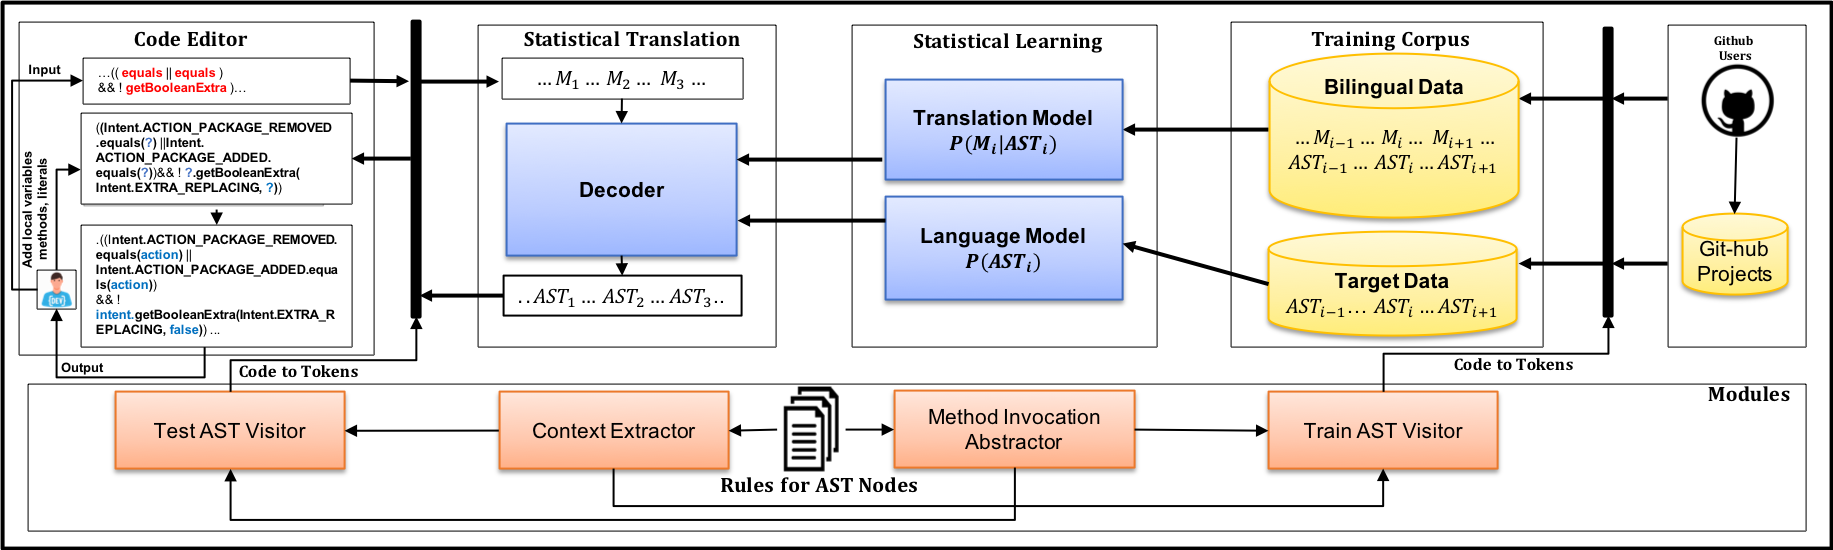
\includegraphics[width=\linewidth]{ApproachOverview.png}
  \caption{Overview Approach of InvocMap }
  \label{fig:ApproachOverview}
\end{figure*}
We summarize the engines inside InvocMap on Figure \ref{fig:ApproachOverview}. From developer view, InvocMap provides a plugin inside with Java code editor to allow (s)he to write a single or multiple method names inside the code environment. From this input, InvocMap translates each method names to respective ASTs. These ASTs reflect the complex structure of method invocations which might be inconvenient for developers to remember. They were abstracted at level 3 in our definition, means they only require developers to add local variables, local methods or literals to get the final code. We will discuss about MI at level 3 of abstraction in the next section. The ability of inferring ASTs for code completion relies on the Statistical Translation module. The training process is done by the Statistical Learning module. This module learns information from the data extracted from large scale Github code corpus  \cite{id:Github}. In general, our statistical approach takes advantages of the knowledge of implementing MIs of experience developers, representing it by a machine learning model to help non-experience developers in retrieving effective implementation of MIs. Both the source code at developers side and code corpus are analyzed to extract sequences of tokens by the Train AST Visitor and Test AST Visitor module we developed. Inside these visitors, we handle each AST Node types by function of modules Context Extractor and MI Abstractor, which we discuss in next sections.
\subsection{Levels of MI Abstraction in InvocMap}
In this section, we describe our theorems for method invocation abstraction.
\begin{definition}
Level 1 of abstraction of a method invocation is the information about method name of that method invocation.
\end{definition}
\begin{definition}
Level 2 of abstraction of a method invocation is the information about type (or signature) of that method invocation.
\end{definition}
\begin{definition}
Level 3 of abstraction of a method invocation is the Abstract Syntax Tree of that method invocation with abstracted place holder for local variables, local methods and literal.
\end{definition}
\begin{definition}
Level 4 of abstraction of a method invocation is the complete Abstract Syntax Tree of that method invocation.
\end{definition}
Along with 4 levels of abstraction in MI, we have the definition of local context provided for each MI. 
\begin{definition}
Local Context of a method invocation is the information about types of local entities and suggested terms. Local entities are local variables, local method invocations and literals inside the MI. The suggested terms are the words that appeared inside the MI.`
\end{definition}

An example of how we see 4 levels is shown in Figure \ref{fig:mapping_expression}. In this code snippet, we have level 1 as method name \texttt{println}. The level 2 of abstraction brings us information about type, which is \texttt{java.io.PrintStream.println}.The level 4 is the final source code which is compilable. The layer 3 is the AST that is having 2 places which are local entities are abstracted by their type information. In the implementation, we represent this AST in level 3 by 4 fields: the code with abstracted places for local entities, the list of types of required arguments to add, the list of imported APIs and the type of MI. These 4 fields will make an unique identification for the expression, which will serve as a representative token for the AST. Because of this, when developer receives an AST at level 3 of abstraction, (s)he will know what types of local variables (s)he can get to get the final code, along with the set of imported APIs. In our work, we focus on the inference from level 1 to level 3 by translation.
We will use information of local context to help developers who already remember what variables should run inside the MI and some words inside the MI to better retrieve the AST of implementation. In Figure \ref{fig:mapping_expression}, we see 2 local entities, including the string literal \texttt{"index"} and the integer variable \texttt{i}. The suggested terms can be \texttt{"System"} and \texttt{"+"} sign. 



\subsection{Levels of Abstraction in Other AST Nodes}
In the context of this work, we call other AST Nodes as all kinds of AST except the MI that are defined in \cite{id:ASTDocumentation}.
\begin{definition}
Level 1 of abstraction of other AST Nodes is the information about the Partial Qualified Name (PQN) of type of those nodes.
\end{definition}
\begin{definition}
Level 2 of abstraction of other AST Nodes is the information about Fully Qualified Name (FQN) of type of those nodes.
\end{definition}
According to definition in \cite{8453132}, an example is the API \texttt{java.io.File}. In this API, we have \texttt{File} as PQN while we have \texttt{java.io.File} as FQN.

\subsubsection{Source and Target Tokens for Other AST Nodes}
We extract information about other AST Nodes to provide useful context for MIs prediction. In the source language, we extract all tokens of level 1 of abstraction for each AST Node, and extract all tokens in level 2 of that AST Node to put into target language. The implementation of the extraction is the Context Extractor module, which is called inside Train AST Visitor and Test AST Visitor. The rules for handling each type of AST are shown in Table \ref{tbl:StatType_rules}. In this Table, the \texttt{PQN()} and \texttt{FQN()} ran when the AST Visitor visit elements that have type. The function for extracting tokens \texttt{S()} and \texttt{D()} can be recursive to sub elements of a given AST Node.

\begin{table}[]
\tiny
\caption{Rules for extract source and target side for AST Nodes }
\centering
\begin{tabular}{|l|Q|}
\hline
\textbf{AST Node }                    & \textbf{Syntax / Source()/ Destination()}                                                                                                 \\ \hline
\multirow{3}{*}{\textbf{Instanceof Expr}}
& E1 instanceof T1                                                               \\ \cline{2-2} 
                &     S(E1) instanceof PQN(T1)                                                                    \\ \cline{2-2}
                &    D(E1) instanceof FQN(T1) 
                     \\
                     \hline
\multirow{3}{*}{\textbf{SimpleName}} & I1                                                               \\ \cline{2-2} 
                &     PQN(I1)                                                                    \\ \cline{2-2}
            &    FQN(I1) 
                     \\
                     \hline
\end{tabular}

\label{tbl:StatType_rules}

\end{table}

\subsubsection{Source and Target Tokens for Method Invocations}
 There are two types of information we want to embed for MI: the mapping between method name and the AST and the information relate to local context. For the first type of information, the source language will store information about token as level 1 of abstraction of MI, while the target language stores information about level 3 of abstraction of MI. Besides, information about local context will be stored by level 1 of abstraction in the source and level 2 of abstraction in the target language. A sequence of tokens for MI in Figure \ref{fig:mapping_expression} is shown in Figure \ref{fig:method_desc_example}.
 
\subsubsection{Method Invocation Abstraction}
We get information about level 3 of abstraction in MI by proposing an algorithm in Listing \ref{lt:AlgorithmMethodAbstractor}. The \texttt{abstractMethodInvocation()} function is invoked when the Train AST Visitor or Test AST Visitor visit a MI and return the abstraction in level 3 by an instance of AST\_Level3 class. This function will use the child class of ASTVisitor called MICVisitor defined in Listing \ref{lt:AlgorithmMethodAbstractor} (Line \#45). This visitor will visit each element inside the MI, check and abstract if the element is a local entity. This visitor also stores other information about the code of AST, the list of required types for each local entities and the set of imported APIs. The handling strategy for each types of AST Node inside the MI is implemented in the \texttt{visitStructure()} function at Line \#61. After visiting and abstracting of MI to an \texttt{AST\_Level3}, this object is checked by the first four fields defined in line \#32 to line \#38 to see if its exist in the dictionary or not. If yes, it will have the id of the existing object in the dictionary. Otherwise, it will generate a new unique id and will be added to the dictionary. The dictionary stores information about abstraction at layer 3 of MIs in the training step. An example of  \texttt{AST\_Level3} object is shown in Figure \ref{fig:mapping_expression}.

\begin{figure}[]
        \center{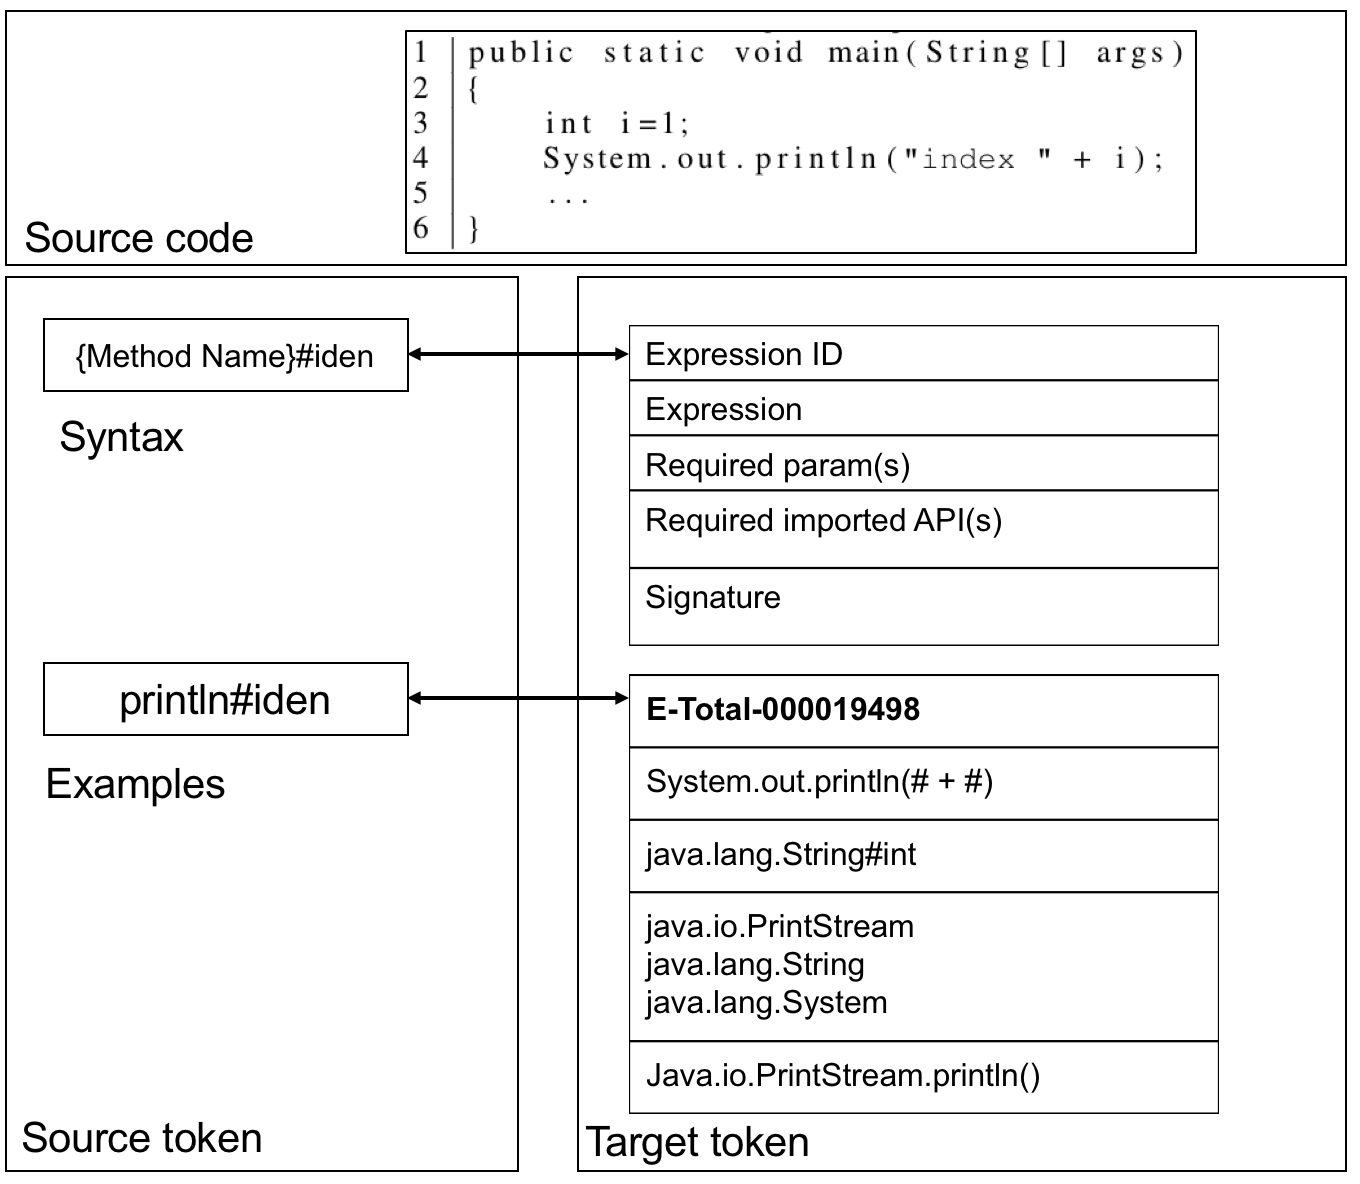
\includegraphics[width=0.4\linewidth]
        {images/example_source_target.png}}
        \caption{\label{fig:mapping_expression} Example of AST\_Level3 instance}
      \end{figure}



\begin{figure}[]
        \center{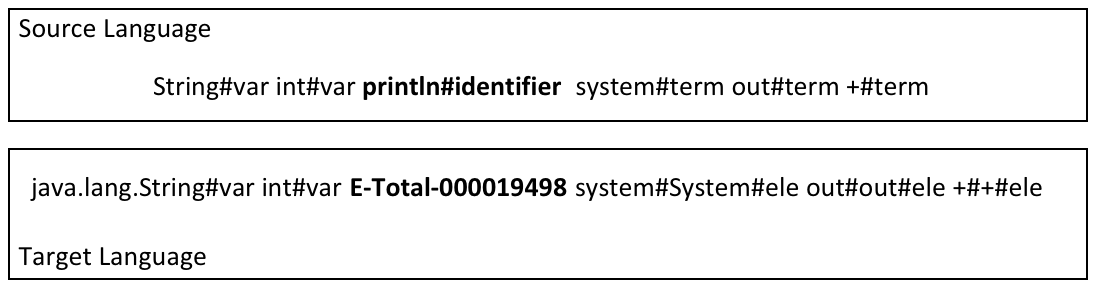
\includegraphics[width=0.4\linewidth]
        {images/methodDescription_example.png}}
        \caption{\label{fig:method_desc_example} Example of tokens for source and target in Method Invocation}
      \end{figure}


\begin{lstlisting}[basicstyle=\tiny,caption={Algorithm for Method Invocation Abstraction},label={lt:AlgorithmMethodAbstractor}]
AST_Level3 abstractMethodInvocation(
		mi : MethodInvocation ,
		dictionaryAST : Set<AST_Level3>,
		visitor : MICVisitor) {
	AST_Level3 result=new AST_Level3(mi);		
	visitor.result=result;
	
	//visit receiver if exist
	Expression receiverExpr=getReceiver(mi);		
	if(receiverExpr not null)
		visitor.visit(receiverExpr);
	
	// add method name and open parenthesis
	result.strCode.append(getMethodName(mi)+"(");
	
	// visit content of arguments
	Expression[] listArguments=getParams(mi);		
	for each Expression argExpr in listArguments:
		visitor.visit(argExpr);
	
	// add close parenthesis
	result.strCode.append(")");

	// set uniqueId
	setUniqueId(result,dictionaryAST);
	
	return result;		
}
...
class AST_Level3 {
	// field to store AST in level 3
	strCode : String;

	// Other informations need to 
	//	add to get final code
	listArguments : List<Type>;
	setImportedAPIs : Set<Type>;	
	strSignature : Type;

	// id is created by the uniqueness of 4 other fields 
	uniqueId : String;
	
}
...
class MICVisitor extends ASTVisitor{
	result : AST_level3;
	...		
	void visit(ASTNode node) {
		/*
		 * If visit local entity,
		 * mark as a place holder
		 * in the AST structure
		 */
		if(isLocalEntity(node)) {
			result.strCode.append("#");
			result.listArguments.append(getType(node));				
		} 
		else  {	
			// visit structure and update result
			// can be recursive if node have children nodes
			visitStructure(node);
		} 			
		// In every cases, add type of node to set of imported APIs
		result.setImportedAPIs.add(getType(node));		
	}	
}
\end{lstlisting}
\subsection{SMT}
To learn the mapping between source and target language, we apply the PBMT \cite{Green2014}. This approach works based on the ability to learn from two models: the language model and the translation model.
\subsubsection{Language Model}
Language Model (LM) plays an important role in a PBMT system. LM is used to predict the next token given a sequence of previous tokens \cite{Koehn:2003:SPT:1073445.1073462}. The more comprehensive corpus of target language do we have, the LM model quality for prediction is higher. LM had been used widely in Software Engineering (SE) researches \cite{Hindle:2012:NS:2337223.2337322,Hel:7180076,Liu:7883371} with potential results. The most basic LM in NLP is uni-gram LM, which calculates the probability of each word based on the number of the appearance of that word in the corpus. This LM provides drawbacks that it doesn't take into account the history of how a word was used in a sequence from previous words. However, if we calculate the probability of a word from all previous words in a sequence of translation, the cost for doing such evaluation is expensive (\cite{Jurafsky:2009:SLP:1214993}). 
\\
Here we use the n-gram language model, which proposed in \cite{Jurafsky:2009:SLP:1214993}. The n-gram LM is used to measure the probability of implementation of MI given a list of previous implementations. The n-gram LM overcome the cost of measuring history for each word by considering and approximate the history for the last n-words that appeared before the current word. Assume that we have m tokens in the target language \({AST_{1},...,AST_{m}}\), the probability provided by LM is:

\begin{equation} 
\tiny
\label{eq:EQ_Probability}
 P[AST_{1}, ...,AST_{m}]=\prod_{i=1}^{m}P[AST_{i} | AST_{i-n},...,AST_{i-1}]
\end{equation}

In equation \ref{eq:EQ_Probability}, the probability for each element of the production on the right side is estimated by the co-occurrence of the current word given the list of the previous words in the target corpus (\cite{Jurafsky:2009:SLP:1214993}). In our model, we use 4-gram LM as the default configuration of LM in NLP.

\subsubsection{Translation Model}
The translation model calculates the probability of a phrase from source language that can be translated to a phrase in a target language. In our problem, if we have a sentence   \({D}\) as the translated result of sentence \({S}\) as tokens in the source language, the selection of \({D}\) as the best candidate is calculated as follows:

\begin{equation} 
\tiny
\label{eq:EQ_Argmax}
 D_{best}=argmax_{D}(p(S|D)*P_{LM}(D)))
\end{equation}

In equation \ref{eq:EQ_Argmax}, \({p(S|D)}\) is the probability of translation model to get the best accuracy calculated by the work of \ref{eq:EQ_ProbTransModel}. In this formula, \(I\) is the number of phrase appeared in sentence \({D}\), while \(\theta ({s_{i}}|{d_{i}})\) is the probability functions between phrase calculated by \cite{Green2014}. Compare to the original translation between natural languages, the translation model in NL has an another type of distribution called reordering distribution. Since our corpus has consistent length between source and target, we don't apply this distribution to equation \ref{eq:EQ_ProbTransModel}.
\begin{equation} 
\tiny
\label{eq:EQ_ProbTransModel}
{p(S|D)=\prod_{i=1}^{I} \theta ({s_{i}}|{d_{i}}) }
\end{equation}



\section{Evaluation}
\textbf{Data Preparation.} To do the evaluation, we select corpus on six well-known libraries. They are Java Development Kit (JDK), Android, GWT, Joda-Time, Hibernate, and XStream. These libraries were selected to generate the corpus for other research works (\cite{8453132,Subramanian:2014:LAD:2568225.2568313}). To generate corpus, we select 1000 highest stars Java projects from Github (\cite{id:Github}), which have most files used API from libraries in Table \ref{tbl:DataPreparation}. For each Java project, InvocMap parses each Java source files by an the Train ASTVisitor module on Figure \ref{fig:ApproachOverview}. The number of pairs respected to each method body we collect is shown in Table \ref{tbl:DataPreparation}. 

\begin{table}[]
\tiny
\caption{Corpus, configurations and RQ3 result}
\label{tbl:CombineConfigTables}
\begin{subtable}[t]{0.1\textwidth}
\centering
\caption{Corpus}
\label{tbl:DataPreparation}
\begin{tabular}{|l|l|}
\hline
\textbf{Library }  & \textbf{Pairs} \\ \hline
JDK       & 820386         \\ \hline
GWT       & 170435         \\ \hline
Joda-Time & 91072          \\ \hline
Android   & 312822         \\ \hline
Hibernate & 149887         \\ \hline
Xstream   & 159170         \\ \hline
\end{tabular}
\end{subtable}
\hfill
\begin{subtable}[t]{0.2\textwidth}
\centering
\tiny
\caption{Configurations}
\label{tbl:Config2}
\begin{tabular}{|l|l|}
\hline
                     & \textbf{Meaning / Example    }                                                                                              \\ \hline
\multirow{2}{*}{\textbf{Config 1}} & Only method name                                                               \\ \cline{2-2} 
                     &  println                                                                   \\ \hline
\multirow{2}{*}{\textbf{Config 2}} &  method name and variables                                                                                       \\ \cline{2-2} 
                         & println 10 5                                        \\ \hline
\multirow{3}{*}{\textbf{Config 3}} & method name, variables and                                                                                  \\ 
 & some suggested words \\\cline{2-2}
               &      println 10 + 5       
                     \\ \hline
Expected &                          
System.out.println(\#+\#)
\\ & Params: int and int     
                     \\ \hline
\end{tabular}
\end{subtable}
\hfill
\begin{subtable}[t]{0.5\textwidth}
\tiny
\flushright
\caption{RQ 3 result}
\begin{tabular}{|l|l|l|l|l|l|}
\hline
              
\textbf{Num }& \textbf{1-10}        & \textbf{11-20}       & \textbf{21-50}       & \textbf{50-100}      & \textbf{\textgreater{}100}     \\
\textbf{of mapping }&         &        &        &       &      \\ \hline
\textbf{Percentage  }   & 12.30\%     & 4.20\%      & 5.96\%      & 4.90\%      & 72.64\%               \\ \hline
\textbf{Accuracy }      & \textbf{Prec}        & \textbf{Prec}        & \textbf{Prec}        & \textbf{Prec}        & \textbf{Prec}                  \\ \hline
GWT            & 96.58\%     & 86.83\%     & 88.71\%     & 86.89\%     & 86.59\%               \\ \hline
Joda-Time      & 93.38\%     & 89.64\%     & 76.19\%     & 69.43\%     & 74.11\%               \\ \hline
JDK            & 98.14\%     & 96.02\%     & 95.26\%     & 91.92\%     & 89.06\%               \\ \hline
Android        & 96.24\%     & 92.51\%     & 90.63\%     & 89.08\%     & 82.58\%               \\ \hline
Hibernate      & 92.61\%     & 87.60\%     & 87.50\%     & 85.47\%     & 78.98\%               \\ \hline
Xstream        & 97.78\%     & 91.01\%     & 78.81\%     & 81.02\%     & 80.80\%               \\ \hline
Total          & 96.47\%     & 93.07\%     & 92.05\%     & 89.41\%     & 87.68\%               \\ \hline
\end{tabular}

\label{tbl:Analyze1}
\end{subtable}

\hfill
\end{table}

\textbf{Training and Testing Configuration.} To train the SMT model, we use a high-end computer with core-i7 Intel processor and use 32 GB of memory. We apply our solution using Phrasal \cite{Green2014}. We allocate Phrasal with phrase length equals to 7. The total training time requires about 6 hours. For testing, we evaluate the ability of translation from a sequence of method names to ASTs in level 3 of abstraction. We simulate 3 configurations sequences of method names regarding to its local context defined in Table \ref{tbl:Config2}. We can see the local context provided for method names is increasing from configurations at level 1 to level 3. At level 1, the input for translation contains only method names with the code context in the source language for translation. It simulates the case that developers write a list of method names inside the code environment. At level 2, information about partial class name of types of local entities is attached along with each method names. This case simulates the case developers remember and write method name and local variables (s)he needs to implement the MI but (s)he doesn't remember the structure of AST. At level 3, each method names in the source language will be attached the information about local entities and half of words appeared inside the MI. This case simulates the case that developers remember some words inside the MI along with local entities. 


\textbf{Metrics.} We evaluate the correct inference of method names. Information about tokens of method name can be recognized by the annotation \texttt{\#identifier} for the source, and the expected results can be recognized by prefix \texttt{"E-Total"} of tokens in the target. We use Precision and Recall as 2 metrics for the evaluation. Out of Vocabulary (OOV) result is the case that the method name token does not in the corpus (Out of Source - OOS) or the expected expression token does not appear in the target corpus (Out of Target - OOT). 
 
\subsection{Research Question (RQ) 1: How InvocMap can perform to predict the implementation with Intrinsic Data?}

  \begin{table}[t]
  \tiny
  \centering
  \caption{Intrinsic Evaluation Result on Github projects and Extrinsic Evaluation Result on Online Forum Code}
\begin{tabular}{|l|l|l|l|l|l|l|l|l|l|l|l|l|l|l|l|l|l|l|}
\hline
          &  \multicolumn{6}{c|}{\textbf{Intrinsic Evaluation with Configuration 1}} &  \multicolumn{6}{c|}{\textbf{Extrinsic Evaluation with Configuration 1}}           \\
\hline
\textbf{Library}   & \textbf{Correct} & \textbf{OOVoc}  & \textbf{Total}   & \textbf{Pre} & \textbf{Rec}  & \textbf{F1} & \textbf{Cor} & \textbf{OOV}  & \textbf{Total}   & \textbf{Pre} & \textbf{Rec}  & \textbf{F1} \\ \hline
GWT       & 39635    & 31522  & 93475   & 63.98\%   & 55.70\% & 59.55\%   & 58              & 9     & 102   & 62.37\%   & 86.57\% & 72.50\%  \\ \hline
Joda-Time & 27364      & 1743   & 39715   & 72.06\%   & 94.01\% & 81.59\%  & 36             & 17    & 75    & 62.07\%   & 67.92\% & 64.86\%  \\ \hline
JDK       & 1053330   & 394317 & 1988644 & 66.07\%   & 72.76\% & 69.25\% & 115            & 44    & 250   & 55.83\%   & 72.33\% & 63.01\%  \\ \hline
Android   & 471347     & 54316  & 617416  & 83.71\%   & 89.67\% & 86.58\% & 51             & 13    & 106   & 54.84\%   & 79.69\% & 64.97\%  \\ \hline
Hibernate & 53319      & 38877  & 117501  & 67.82\%   & 57.83\% & 62.43\% & 125            & 40    & 226   & 67.20\%   & 75.76\% & 71.23\%  \\ \hline
Xstream   & 4671      & 3019   & 9382    & 73.41\%   & 60.74\% & 66.48\%  & 44             & 14    & 64    & 88.00\%   & 75.86\% & 81.48\%  \\ \hline
Total     & 1649666   & 523794 & 2866133 & 70.43\%   & 75.90\% & 73.06\%   & 429           & 137   & 823   & 62.54\%   & 75.80\% & 68.53\%  \\ \hline
          & \multicolumn{6}{c|}{\textbf{Intrinsic Evaluation with Configuration 2}}  & \multicolumn{6}{c|}{\textbf{Extrinsic Evaluation with Configuration 2}}   \\
\hline
GWT       & 53042                                     & 31522  & 93475   & 85.62\%   & 62.72\% & 72.40\%    & 88              & 9     & 102   & 94.62\%   & 90.72\% & 92.63\%  \\ \hline
Joda-Time & 29028                                     & 1743   & 39715   & 76.45\%   & 94.34\% & 84.45\%  & 53             & 17    & 75    & 91.38\%   & 75.71\% & 82.81\% \\
\hline
JDK       & 1347221                                    & 394359 & 1988644 & 84.50\%   & 77.36\% & 80.77\%  & 177            & 44    & 250   & 85.92\%   & 80.09\% & 82.90\%  \\
\hline
Android   & 470725                                    & 54321  & 617416  & 83.60\%   & 89.65\% & 86.52\% & 85             & 13    & 106   & 91.40\%   & 86.73\% & 89.01\%  \\
\hline
Hibernate & 63275                                     & 38881  & 117501  & 80.48\%   & 61.94\% & 70.00\% & 138            & 40    & 226   & 74.19\%   & 77.53\% & 75.82\%  \\
\hline
Xstream   & 5145                                      & 3019   & 9382    & 80.86\%   & 63.02\% & 70.83\% & 49             & 14    & 64    & 98.00\%   & 77.78\% & 86.73\%  \\
\hline
Total     & 1968436                                   & 523845 & 2866133 & 84.04\%   & 78.98\% & 81.43\%   & 590           & 137   & 823   & 86.01\%   & 81.16\% & 83.51\%     \\
\hline
          & \multicolumn{6}{c|}{\textbf{Intrinsic Evaluation with Configuration 3}}      & \multicolumn{6}{c|}{\textbf{Extrinsic Evaluation with Configuration 3}}            \\
\hline
GWT       & 55510                                     & 31522  & 93475   & 89.60\%   & 63.78\% & 74.52\%    & 89              & 9     & 102   & 95.70\%   & 90.82\% & 93.19\%  \\
\hline
Joda-Time & 31394                                     & 1743   & 39715   & 82.68\%   & 94.74\% & 88.30\%  & 55             & 17    & 75    & 94.83\%   & 76.39\% & 84.62\%  \\
\hline
JDK       & 1435424                                    & 394359 & 1988644 & 90.04\%   & 78.45\% & 83.84\%  & 174            & 44    & 250   & 84.47\%   & 79.82\% & 82.08\%  \\
\hline
Android   & 498708                                    & 54321  & 617416  & 88.57\%   & 90.18\% & 89.36\% & 82             & 13    & 106   & 88.17\%   & 86.32\% & 87.23\%  \\
\hline
Hibernate & 65860                                     & 38881  & 117501  & 83.77\%   & 62.88\% & 71.84\% & 146            & 40    & 226   & 78.49\%   & 78.49\% & 78.49\%  \\
\hline
Xstream   & 5516                                      & 3019   & 9382    & 86.69\%   & 64.63\% & 74.05\% & 50             & 14    & 64    & 100.00\%  & 78.13\% & 87.72\%  \\
\hline
Total     & 2092412                                   & 523845 & 2866133 & 89.33\%   & 79.98\% & 84.40\%   & 596           & 137   & 823   & 86.88\%   & 81.31\% & 84.00\%   \\
\hline
\end{tabular}

\label{tbl:IntrinsicAndExtrinsic}
\end{table}


We split the pairs of our parallel corpus for training and testing. We get 10\% of the data for testing and the other with training and do ten-fold cross-validation to test the ability of prediction on our full data set. In total, there are 2.86 Million of MIs collected from 1000 projects from Github \cite{id:Github}.
The evaluation result for intrinsic data is shown in Table \ref{tbl:IntrinsicAndExtrinsic}. We show that from configuration 1 to configuration 3, the F1 score increases from 73.06\% to 84.4\%. This seems to be feasible, since the fact that if we provide more local context information along with method names, the ability to predict correctly AST in level 3 for the translation model is better. We see one observation is that the number of Out of Vocabulary expressions are higher in percentage, cause decreasing in recall compare to the research work that applied Machine Translation for inferring Fully Qualified Name from incomplete code (\cite{8453132}). This is reasonable, since our work requires to infer the MI in level 3 of abstraction, which contains detail structure compared to output of \cite{8453132} as type information of MIs. 

We study an example in the Intrinsic Evaluation in Figure \ref{fig:example_in}. This example is a function collected from \cite{id:IntrinsicAndroidExample} from our corpus. The testing for intrinsic evaluation simulates the case developers input only \texttt{println} inside the code environment, the output of this case will be the implementation of \texttt{java.io.PrintWriter.println()} function. We can see that the surrounding code is useful to infer the correct expression. If we do not have the context information, which means developer input \texttt{println} in an empty method, the translated result will return the most popular MI, \texttt{System.out.println()}.

\subsection{RQ2: How well InvocMap can perform to predict the implementation with Extrinsic Data?}

To do this experiment, we collect the data as code snippets from Online Forums (\cite{id:StackOverflow,id:ProgramCreek,id:GeeksForGeeks}). To do this, a Software Engineer who has 5 years of experience in Java programming was hired to collect code snippets from 120 posts in Online Forums, with 20 posts for each library in Table \ref{tbl:DataPreparation}. The result for extrinsic evaluation is shown in Table \ref{tbl:IntrinsicAndExtrinsic}. We see that with level 1, since the case that only method names are provided in the source language, our approach stills predict correctly 62.54\% in precision. With the configuration levels that developers add more information, the precision increases to 86.88\%. For each library, we achieved the highest accuracy on GWT and lowest on Hibernate with input as detail information like configuration 3. This result seems reasonable, since Hibernate is a bigger library compared to GWT but it is not as popular as JDK, causes the variety of ASTs for APIs in this library.

\subsection{RQ3: How well InvocMap can perform to predict ambiguous method names?}

In this evaluation, we analyze the relation of the expression prediction result relates to the number of mapping of each method name from the parallel corpus. We use data collected for the Intrinsic Evaluation with configuration 3. The result is shown in Table \ref{tbl:Analyze1}, which shows that from the number of method name that has more than 100 mappings in the parallel corpus are about 72\% of the total data. It proves the complexity of kinds of implementation for each method names. The total precision tends to decrease from 96.47 \% to 87.68\%. This proves the ability to generate expression from input queries.









\section{Discussion}
There are some threats to validity of our work. First, the data might not be representative. To alleviate this threat, we select high quality Github projects for training by selecting highest stars project which uses six popular libraries and select reliable online forums to get the code corpus.  Second, we evaluate the accuracy of the translation system automatically. We consider the input for translation as all method names and evaluate the accuracy of their respected ASTs. In reality, developers might write full implementation of MI if (s)he remembered how to implement that function along with writing method names in case they need suggestion. Thus, the method names of already implemented MIs can be skipped if we consider about the accuracy of the inference of method names that developers need the suggestion. We will hire people to set up this type of evaluation in future.\\
There are a few challenges that we need to improve for the translation. First, we still require developers to remember the method names for the inference. This could be a challenges for developers at a very beginning level of expertise. We consider that the more appropriate input can be Natural Language (NL) text descriptions by developers instead of method names and local entities. An interesting future work should be extending the original SMT model to accept natural language description by processing the description to have the most appropriate method names and local entities automatically for the input of method name to AST translation.  Second, since in reality developers can write the full MIs along with method names, InvocMap still doesn't take advantage of information provided by implemented MIs. This brings us to improve our work by a specific Machine Translation research for the case that some of source tokens we already know the result, and how we use those information to increase the accuracy, which can be useful  in applying SMT in other areas. Third, our SMT model still not be able to generate the MI at the fully details level. We will combine SMT with program analysis for the inference from level 1 to level 4 of MIs in future works. 
\section{Related Works}
Machine Learning has been applied widely in Software Engineering applications \cite{Allamanis:2018:SML:3236632.3212695}. Generating code by machine learning is an interesting but also confront challenges. There is a research by \cite{DBLP:journals/corr/BaroneS17} shows that the inference of code from documentation by machine translation achieved very low accuracy results on both SMT and Neural Machine Translation (NMT) models learned from practical large scale code corpus. There are two reasons cause this challenges. First, large scale code corpus contains noise data \cite{Pascarella:2017:CCC:3104188.3104217}. Second, the structure of AST Node is complicate for a machine translation system to learn about the syntactically correct of generated code as shown in \cite{DBLP:journals/corr/BaroneS17}. \cite{Gu:2016:DAL:2950290.2950334} propose an approach to achieve the implementation from  in natural language description. However, the output of their tool consists only sequence of APIs which is in level 2 of our abstraction for MIs. In our work, we target the inference of MI in level 3 with the ability of complex AST structure of MIs.
\\
There are several other inputs to get the complete code in other researches. \cite{7372046} derive the code in C\# language from code in Java language by machine translation. \cite{Gvero:2015:SJE:2814270.2814295,Gu:2016:DAL:2950290.2950334} generate the code from natural language descriptions. In these works, they consider the textual description as the full information for the inference. We consider our code generation problem in a different angle, which we take advantage of the surrounding context along with the textual description of method name in our work. \cite{6227236} propose a graph based code completion tool that suggest the full code snippet when developers are writing an incomplete code. This work focuses on completing the code from a part of the code. We propose an inference from the skeleton of method invocations, which is in form of sequence of method names, to the implementation of method invocations.
\section*{Conclusion}
In this work, we proposed InvocMap, a SMT engine for inferring
the ASTs of method invocations from a list of method
names and code context. By the evaluation on corpus
collected from Github projects and online forums, we demonstrated
the potential of our approach for auto code completion. A major
advantage of InvocMap is that it is built on the idea of abstracting
method invocations by four different levels. We provided an algorithm
to achieve AST of method invocations for the method invocations inference. As
future works, we will work on extending the SMT model to
support inputs from multiple natural language descriptions of
multiple method invocations, along with investigation of machine learning techniques for improving the accuracy. 





\clearpage
\bibliography{refs}
\bibliographystyle{iclr2020_conference}



\end{document}
